\subsection{Protocolo de prueba}

\subsubsection{Evaluación del modulo: PROCESAMIENTO DE IMÁGENES}

Existe distintas formas de evaluar un modelo de detección de objetos. Algunas de ellas son: 

\paragraph{Matriz de confusión}\mbox{}\\

Cada fila de la matriz representa el numero de predicciones de cada clase, mientras que cada columna representa el verdadero valor. Se evalúan todos los resultados y se dividen en verdaderos positivos, falsos negativos, falsos positivos y verdadero negativo.\par
\bigbreak
\begin{tabular}{l|l|c|c|}
\multicolumn{2}{c}{}&\multicolumn{2}{c}{Valor verdadero}\\
\cline{3-4}
\multicolumn{2}{c|}{}&Tomate&Next\\ 
\cline{2-4}
\multirow{2}{*}{Valor predicho}& Tomate & Verdadero Positivo (VP) & Falso Positivo (FP)\\
\cline{2-4}
& Next & Falso Negativo (FN) & Verdadero Negativo (VN)\\
\cline{2-4}
\end{tabular}
\bigbreak
\begin{itemize}
    \item Verdaderos positivos (VP): Predicciones correctas respecto a los datos verdaderos.
    \item Falso positivo (FP): Se detecta una clase que no existe en los datos verdaderos.
    \item Falso Negativo (FN): Una clase se detecta como otra clase o simplemente no se detecta pero si existe en los datos.
    \item Verdadero Negativo (VN): Una clase que no se detecta o se detecta como otra y no existe en los datos. 
\end{itemize}
\bigbreak

\subparagraph{Métrica}\mbox{}\\

\subparagraph{Precisión}
La precisión mide el porcentaje de predicciones positivas correctas entre todos los casos positivos que existen.

\[Precisión = \frac{VP}{VP+FP}\]

\subparagraph{Sensibilidad}
La sensibilidad (Recall) mide las predicciones positivas correctas entre todas las predicciones hechas.

\[Sensibilidad = \frac{VP}{VP+FN}\]

\subparagraph{Exactitud}
Pocentaje total de los aciertos del modelo.

\[Exactitud = \frac{TP+TN}{TP+TN+FP+FN}\]

\paragraph{Intersección sobre unión}\mbox{}\\

Mide la precisión de un detector en un conjunto de datos en particular.

\begin{center}
    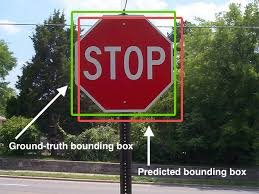
\includegraphics[scale=0.7]{Tesis/Capitulos/07_RESULTADOS/fig/IoU.jpeg}
    \captionof{figure}{Ejemplo IoU}
\end{center}

\[IoU = \frac{\text{Área de solapamiento}}{\text{Área de unión}}\]

Donde, ''Área de solapamiento'' entre la predicción y la realidad, mientras que el ''Área de unión'' es el área sumada entre la predicción y la realidad.

\paragraph{Precisión promediada (AP: Average Precision)}\mbox{}\\

Es una métrica comúnmente utilizada como resumen de una curva que forma la relación entre dos métricas, la Precisión y la Sensibilidad de la red.\par

\begin{center}
    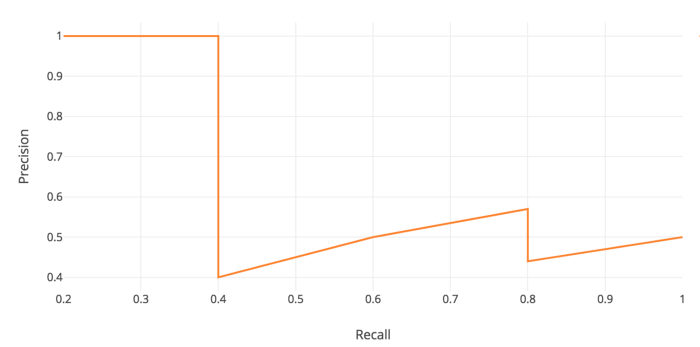
\includegraphics[scale=0.5]{Tesis/Capitulos/07_RESULTADOS/fig/PrecisionSensibilidad.png}
    \captionof{figure}{Precisión-Sensibilidad}
\end{center}

Algo a tener en cuenta es que la curva es decreciente ya que si uno entrena a su clasificador para aumentar la precisión, la sensibilidad disminuirá.\par
Como por definición la precisión promediada (AP) es el área bajo la curva y queremos hacer mas sencillo el proceso, antes de calcular la precisión promediada, ponderamos la curva.\par

\begin{center}
    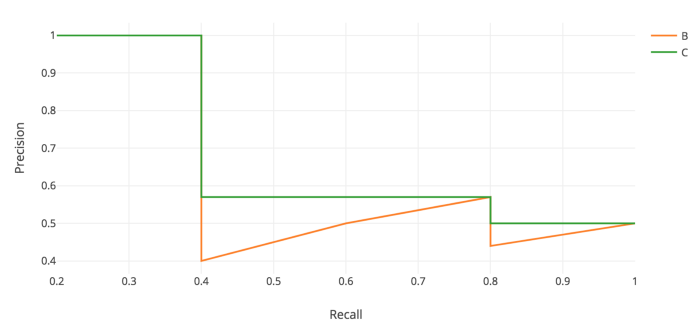
\includegraphics[scale=0.5]{Tesis/Capitulos/07_RESULTADOS/fig/PrecisionSensibilidadSuave.png}
    \captionof{figure}{Precisión-Sensibilidad ponderada}
\end{center}

Matemáticamente se calcula, para aquellas predicciones consideradas correctas (IoU mayor a un determinado threshold), como:

\[AP = \sum_{}^{}(r_n - r_{n-1}) P_{interp(r_n)} \]

Donde $r_n$ es la sensibilidad para un determinado valor de IoU. Y $p_{interp}(r) = max_{r>r_n} p(r)$ ya que gráficamente reemplazamos cada valor de precisión con el valor máximo de precisión a la derecha de ese nivel de Sensibilidad.

\paragraph{Precisión promediada media (mAP: Mean Average Precisión)}\mbox{}\\

Si el conjunto de datos contiene N clases:

\[mAP = \frac{1}{N}  \sum_{class=1}^{N}(AP_{class})  \]

\paragraph{Sensibilidad promediada (AR: Average Recall)}\mbox{}\\

En vez de calcular la Sensibilidad en un valor particular de IoU, calculamos la Sesnbilidad promediada (AR) con IoU desde 0.5 a 1.
Matemáticamente AR es definido como: 

\[ AR = 2 \int_{0.5}^{1} recall(IoU) \,d(IoU)  \]

\paragraph{Sensibilidad promediada media (mAR: Mean Average Recall)}\mbox{}\\

Si el conjunto de datos contiene N clases:

\[ mAR = \frac{ \sum_{i=1}^{K}(AR_{i})  }{ K}  \]

\paragraph{Puntaje F1 (F1 score)}\mbox{}\\

El valor F1 combina las medidas de Precisión y Sensibilidad en un solo valor. Esto resultas practico ya que en un solo valor se puede comparar el rendimiento combinado por la Precisión y la Sensibilidad.

\[ F1 = 2 \times \frac{Precisión \times Sensibilidad}{Precisión+Sensibilidad} \]


\subsubsection{Evaluación del modulo: SISTEMA DE CONTROL DIFUSO}

A partir de la simulación desarrollada se podrá chequear el funcionamiento del sistema, y reglas de control difuso.\par
Además se realizarán múltiples pruebas testeando el sistema de control difuso. Se colocaran obstáculos frente al robot en todas las distancias posibles según las etiquetas lingüísticas de las variables de entrada (cerca, lejos) y se evaluara la salida del sistema (ángulo a corregir) buscando obtener otra vez, todas las etiquetas lingüísticas de las variables de salida (izquierda, centro, derecha).